%%%%%%%%%%%%%%%%%%%%%%%%%%%%%%%%%%%%%%%%%%%%%%%%%%%%%%%%%%%%%%%%%%%%%%%%%%%%%%%
%
% Tommy P. Keane
% Master of Science Thesis
% Department of Electrical and Microelectronic Engineering
% Rochester Institute of Technology
%
% April 2011
%
%
%
% Funded By: Lenel Systems Inc., A UTC Fire & Security Corporation
%
% Algorithm Intellectual Property Owned By: Lenel Systems Inc.
%
%
% http://www.tommypkeane.com
%
%%%%%%%%%%%%%%%%%%%%%%%%%%%%%%%%%%%%%%%%%%%%%%%%%%%%%%%%%%%%%%%%%%%%%%%%%%%%%%%

%%%%%%%%%%%%%%%%%%%%%%%%%%%%%%%%%%%%%%%%%%%%%%%%%%%%%%%%%%%%%%%%%%%%%%%%%%%%%%%
%
% CHAPTER 4
%
% SECTION 1: Affine Views
%
%%%%%%%%%%%%%%%%%%%%%%%%%%%%%%%%%%%%%%%%%%%%%%%%%%%%%%%%%%%%%%%%%%%%%%%%%%%%%%%


%%%%%%%%%%%%%%%%%%%%%%%%%%%%%%%%%%%%%%%%%%%%%%%%%%%%%%%%%%%%%%%%%%%%%%%%%%%%%%%
% BEGIN DOCUMENT

The rooftop scene, Figure \ref{RooftopImages}, is a view from the Tufts University campus in Massachussetts. As mentioned, this is a large image that has been cropped into two overlapping views. By testing the WFMI algorithm with these two ideal views (and other similar scenarios) a better understanding of the feature generation, entropy concerns, and overlap limitations for the algorithm were found. Through empirical testing of affine views of realistic (but affine) scenes it was found that a minimum of 10\% pixel overlap could be tolerated on average. As the entropy of  the scene in the overlap region increases, more distinct and varied features can be generated, and the less overlap that is required between the views. This directly follows from the implementation of the WFMI metric which calculates similarity based on the distributions of features in the overlap regions. Scenes with large amounts of entropy will have very distinct features that will have a low probability of reoccurring elsewhere in the scene, and thus elsewhere in any of the views besides in the overlap region. In an extremely unrealistic, high entropy, case it was found that the WFMI algorithm can register views with only 1\% of the total pixels overlapping. To provide a general metric, realistic affine views (views similar to surveillance views, such as the Rooftop views) of a purely affine scene were found to require a minimum of 10-15\% of the total number of pixels be in the overlap region.

The automatically blended rooftop views in Figure \ref{RooftopStitched} can be compared to the manually blended views in Figure \ref{RooftopStitchedManual}. The manual blending technique follows the WFMI algorithm's multi-resolution spline blending algorithm but the affine homography is generated by MATLAB\textsuperscript{\textregistered}'s feature correspondence selection tool (\textit{cpselect}) and the correspondence to transform function (\textit{cp2tform}). These views were produced with roughly 16\% of the pixels from each view occurring in the overlap region. This is a relatively low entropy scene as there are very large areas of flat texture (concrete, glass, sky, trees, \etc).

As can be seen in Figure \ref{RooftopStitchedManual} there is a rotation disparity from the manual results and the stitching seam is clearly visible as the views have been misregistered. In order to attempt to compare the algorithm to the manual method in terms of practical implementation, the feature points for the manual transform derivation were chosen relatively quickly at the building and window corners. There were 12 to 15 points chosen and they were automatically passed into the least-squared algorithm in MATLAB\textsuperscript{\textregistered}'s \textit{cp2tform} function. The idea was that if a user could choose accurate points in a comparable amount of time for the computation of the automated registration then the automated registration could be compared to the current system in place by the grant provider. This is not a rigorous test, but it shows that even for an affine view, point-to-point correspondence has far less tolerance for error.

To show the aforementioned statistical errors that can occur and why the filtering operation is a crucial and useful addition to basic MMI algorithms, the views in Figure \ref{RooftopNoisyImages} were degraded by additive white Gaussian noise resulting in an average SNR between the two views of roughly 24 dB. The degradation is clearly visible and will surely affect the calculation of the color gradients. The maps in Figure \ref{RooftopNoisyImagesMI} are the AFNMI (left) and NMI maps for the registration of the noisy images. Clearly there is a large peak in the NMI map towards the center, but a smaller sharper peak off to the left side, as shown. This smaller peak is the true translation, but it would go undetected in a normal MMI implementation. As shown in the AFNMI map, it is extracted as the true peak, far above any other possibility. These maps are shown normalized to the height of their peak, the actual scale is not visually useful and would have only added confusion.

An alternate affine set of views is presented in the stone wall scene. This is again a single view of a realistic scene with two overlapping affine views cropped from the larger view. This is a view of a wall and warehouse in Allston, MA. These views have only 10\% of the total image pixels in the overlap and are registered perfectly by the automatic WFMI algorithm. While they seem to be a generally low entropy pair of images, they are extremely different in their content. Only in the overlap region is there a rectangular region that corresponds, based on the shadow and the stones present in the views. This allows a much smaller overlap, despite the lack of entropy, and where point correspondence may be easily confused by the low entropy metal siding of the building (repeated pattern), the WFMI algorithm is a structural search that is extremely robust in such cases.

Again to show the strength of the algorithm, noise has been added to the images, this time though the registration can stay accurate down to an average SNR of roughly 16 dB because of the uniqueness of the overlap region between the views.

Lastly, to show the accuracy of the affine case, a cropped scene of the Stone Wall was modified to only have 1\% of the pixels in each view be part of the overlap region and the accuracy is maintained. Blending errors from the image padding as discussed in the previous chapter are visible near the top of the image as there is an increase in brightness with no apparent source. Again, that is an implementation artifact (as in, the choice of the means of implementation) not an error in the design or algorithm, and not an error in that it was implemented incorrectly.

% ROOFTOP
\begin{figure}
\label{RooftopImages}
\centering
\subfigure{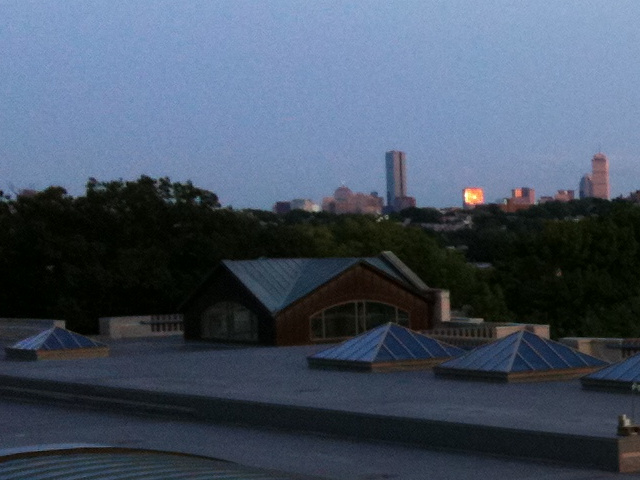
\includegraphics[width=.45\textwidth]{RooftopL001} \label{RooftopL}}
\subfigure{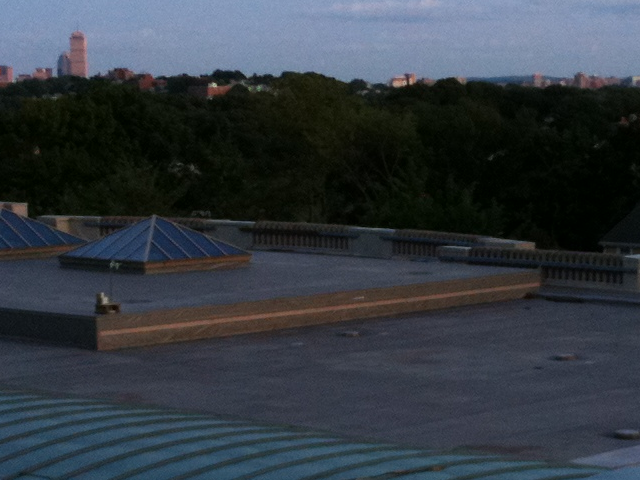
\includegraphics[width=.45\textwidth]{RooftopR001} \label{RooftopR}}
\caption{Rooftop Views (a) Left View, (b) Right View}
\end{figure}

\begin{figure}
\centering
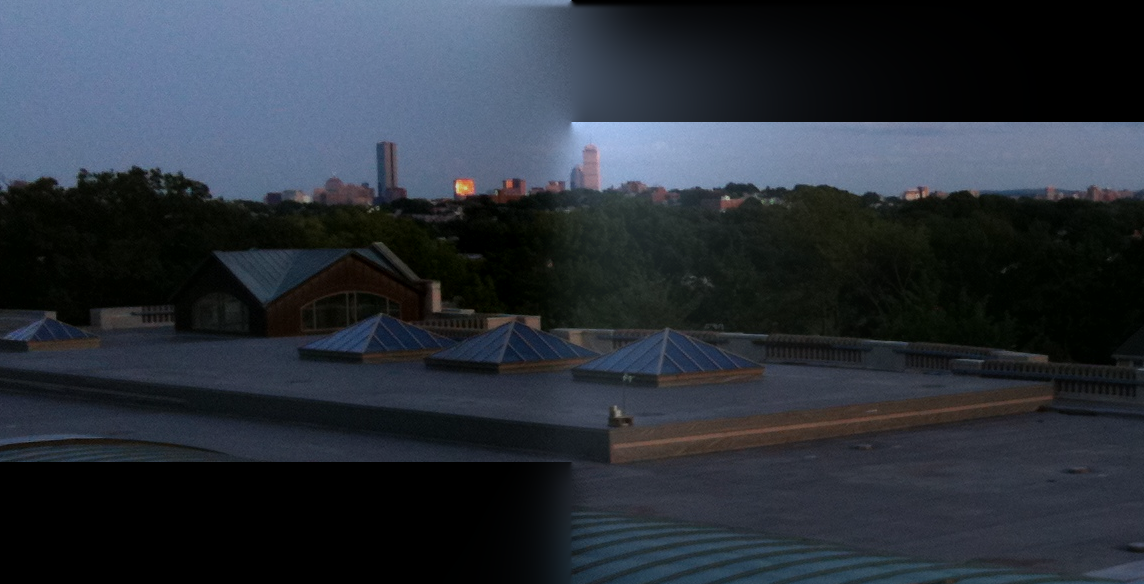
\includegraphics[width=1\textwidth]{RooftopSP001001}
\caption{Rooftop Views Blended}
\label{RooftopStitched}
\end{figure}

\begin{figure}
\centering
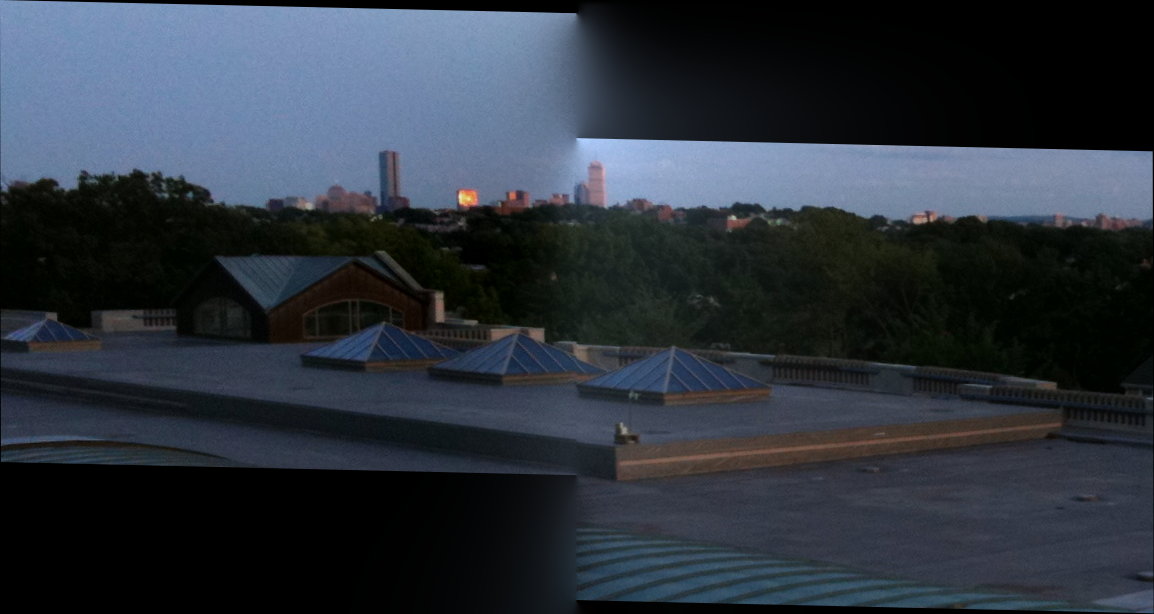
\includegraphics[width=1\textwidth]{RooftopSP001ManAff}
\caption{Rooftop Views Blended Manually (Affine)}
\label{RooftopStitchedManual}
\end{figure}

% ROOFTOP NOISE
\begin{figure}
\centering
\subfigure{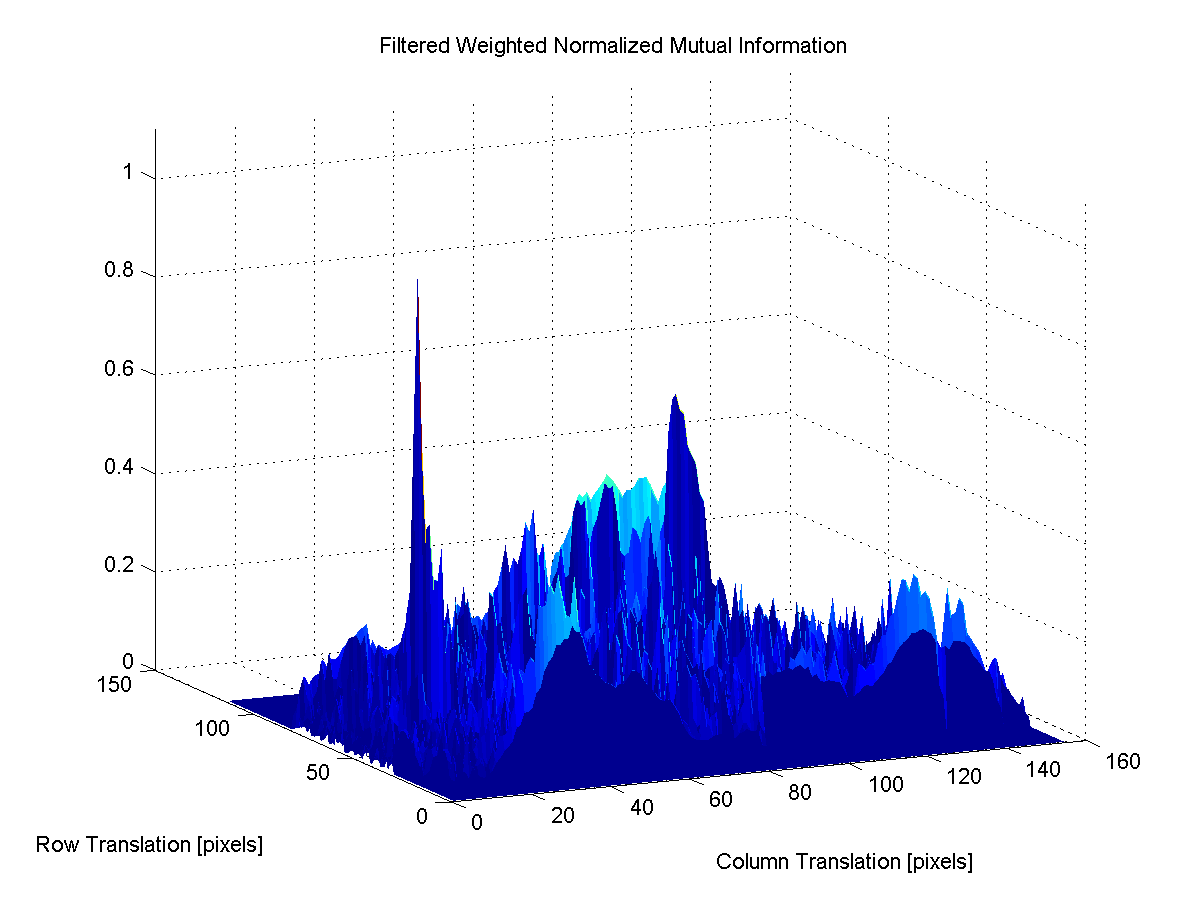
\includegraphics[width=.49\textwidth]{RooftopNoisy24122001FWNMI} \label{RooftopNoisy24122001FWNMI}}
\subfigure{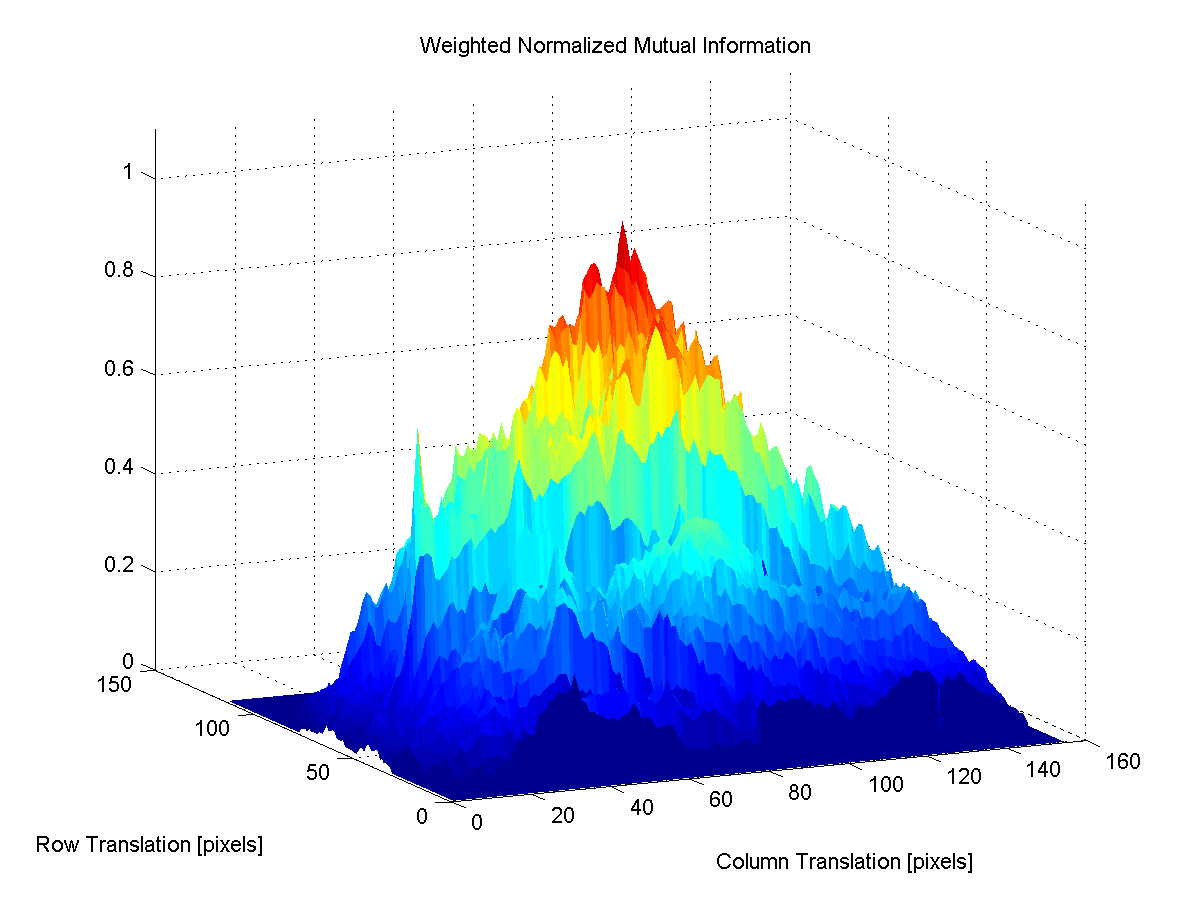
\includegraphics[width=.49\textwidth]{RooftopNoisy24122001WNMI} \label{RooftopNoisy24122001WNMI}}
\caption{Mutual Information Maps from Translation Search (a) Filtered and Weighted, (b) Weighted}
\label{RooftopNoisyImagesMI}
\end{figure}

\begin{figure}
\centering
\subfigure{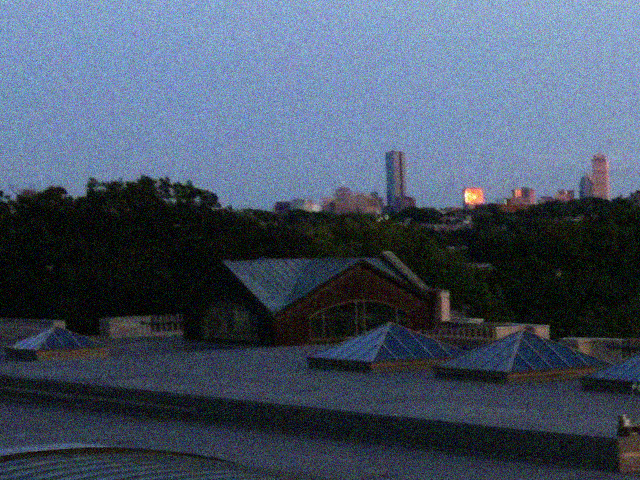
\includegraphics[width=.45\textwidth]{RooftopNoisy24122L001} \label{RooftopNoisy24122L001}}
\subfigure{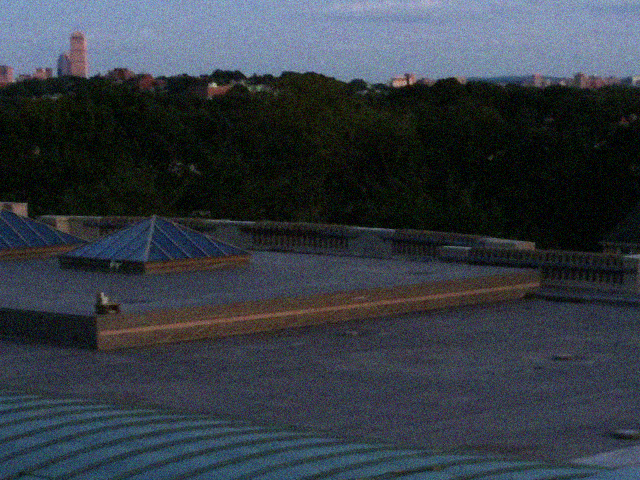
\includegraphics[width=.45\textwidth]{RooftopNoisy24122R001} \label{RooftopNoisy24122R001}}
\caption{Rooftop Views with Average SNR of 24.122 dB (a) Left View, (b) Right View}
\label{RooftopNoisyImages}
\end{figure}

\begin{figure}
\centering
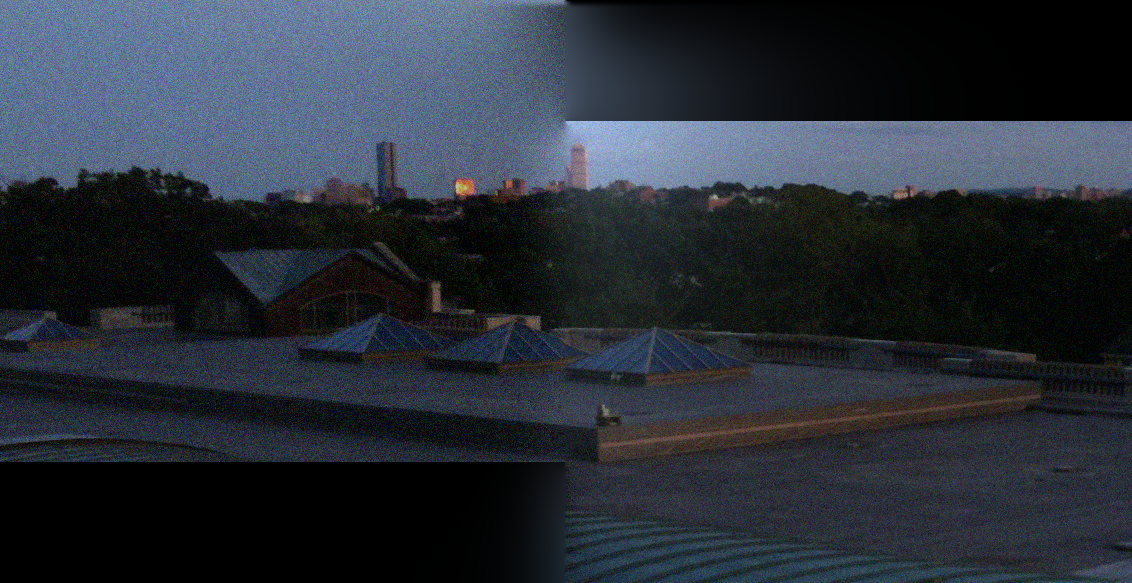
\includegraphics[width=1\textwidth]{RooftopNoisy24122SP001001}
\caption{Rooftop Noisy Views Blended (Average SNR: 24.122 dB)}
\label{RooftopNoisyStitched}
\end{figure}

% STONE WALL
\begin{figure}
\label{StoneWallImages}
\centering
\subfigure{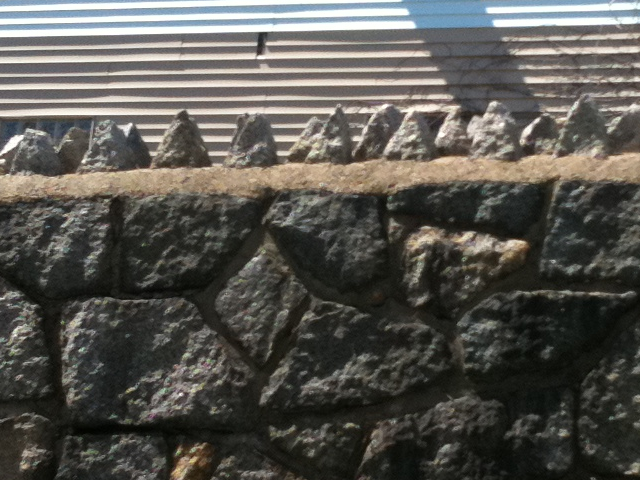
\includegraphics[width=.45\textwidth]{StoneWallL001} \label{StoneWallL}}
\subfigure{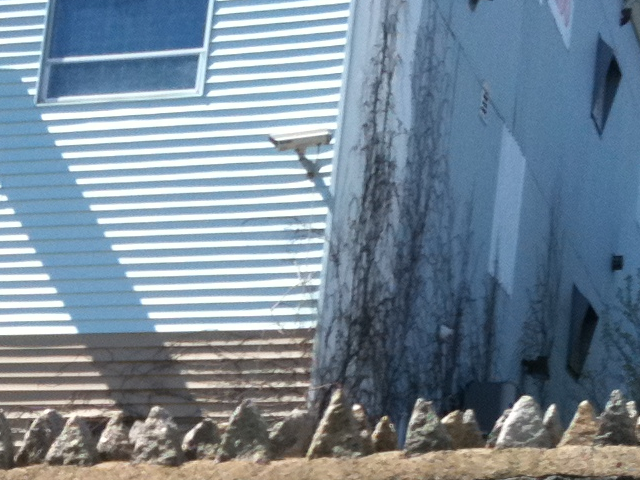
\includegraphics[width=.45\textwidth]{StoneWallR001} \label{StoneWallR}}
\caption{Stone Wall Scene (a) Left View, (b) Right View}
\end{figure}

\begin{figure}
\label{StoneWallStitched}
\centering
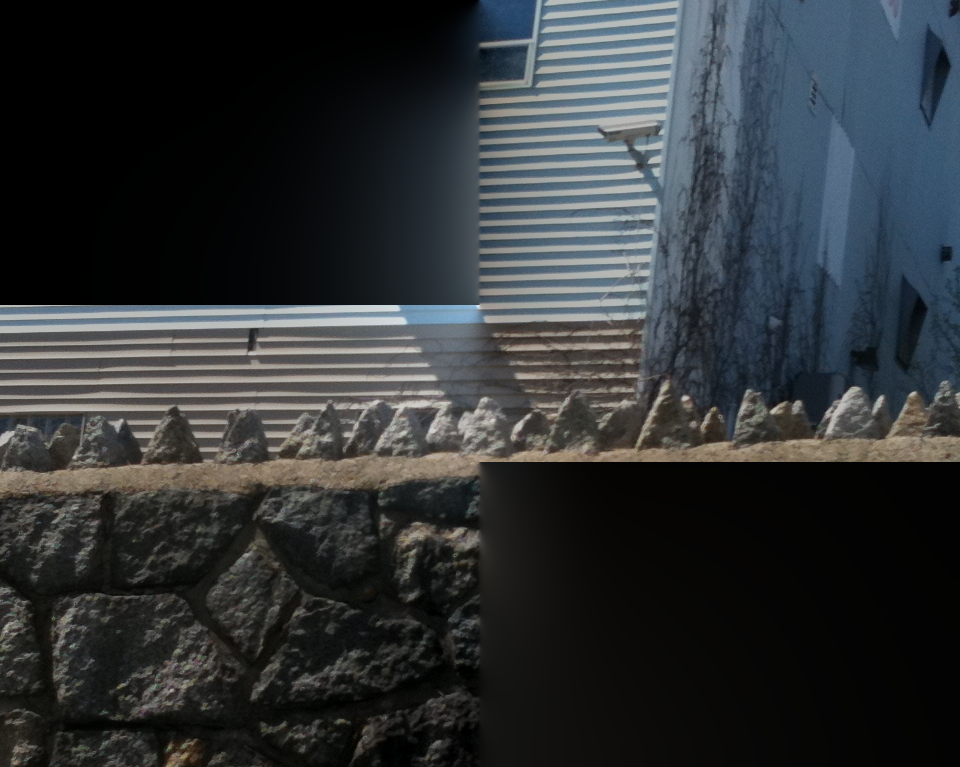
\includegraphics[width=1\textwidth]{StoneWallSP001001}
\caption{Stone Wall Views Blended}
\end{figure}

% STONEWALL NOISE
\begin{figure}
\centering
\subfigure{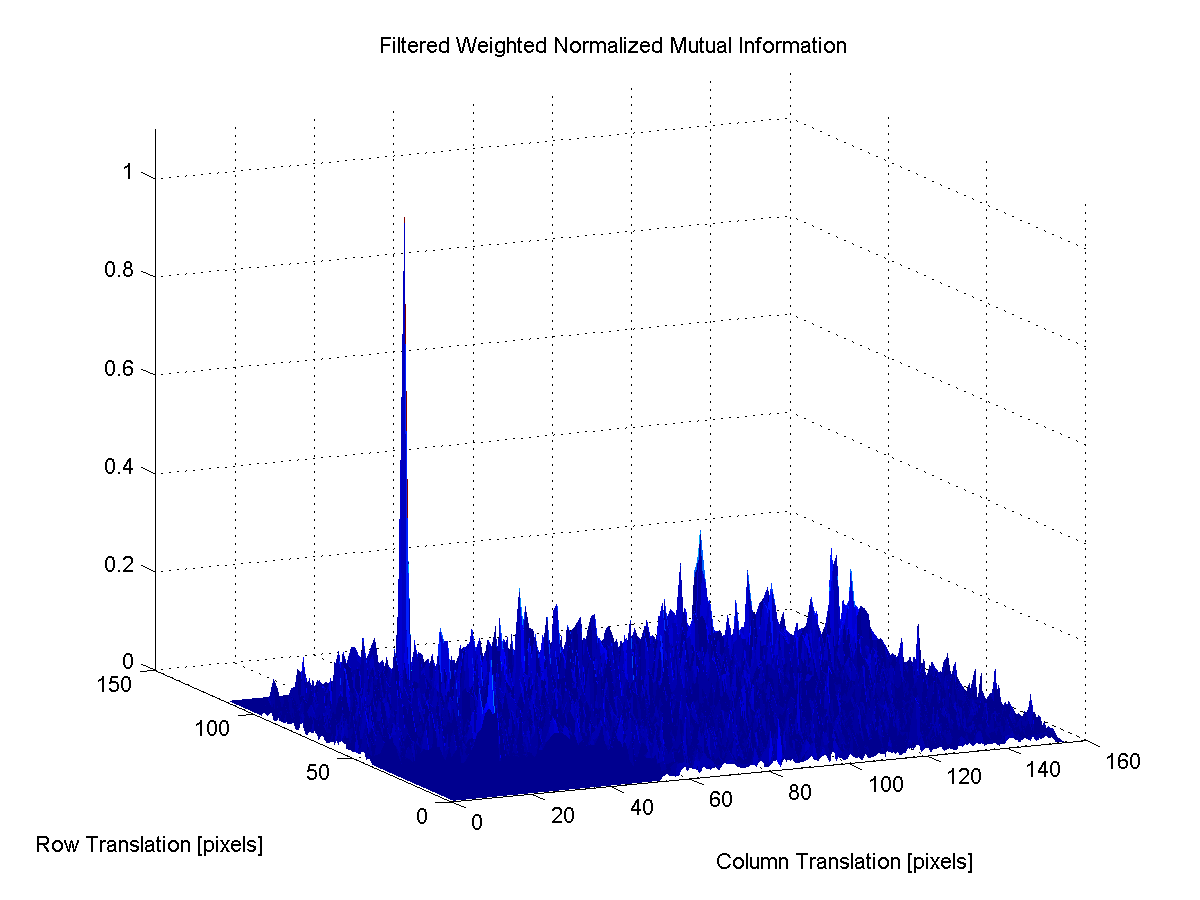
\includegraphics[width=.49\textwidth]{StoneWallNoisy164725001FWNMI} \label{StoneWallNoisy164725001FWNMI}}
\subfigure{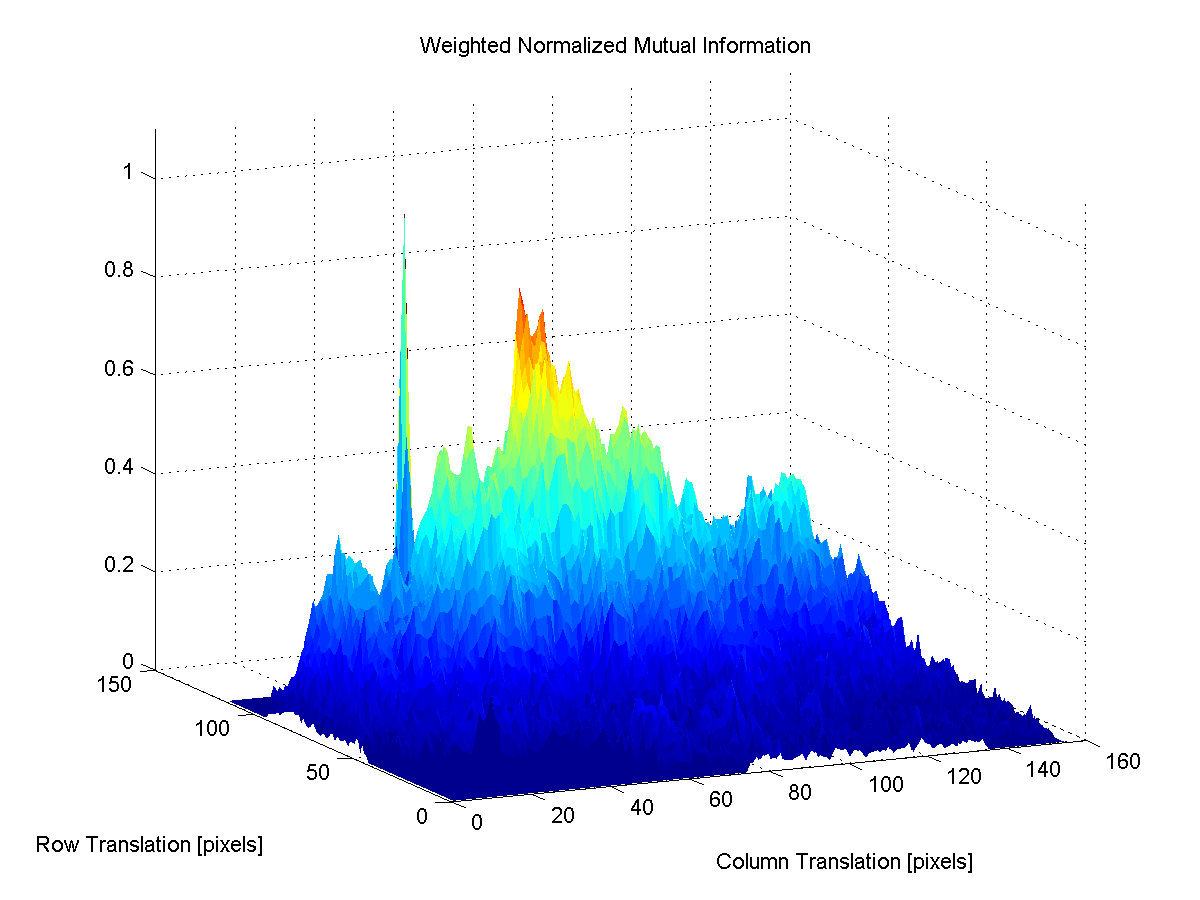
\includegraphics[width=.49\textwidth]{StoneWallNoisy164725001WNMI} \label{StoneWallNoisy164725001WNMI}}
\caption{Mutual Information Maps from Translation Search (a) Filtered and Weighted, (b) Weighted}
\label{StoneWallNoisyImagesMI}
\end{figure}

\begin{figure}
\centering
\subfigure{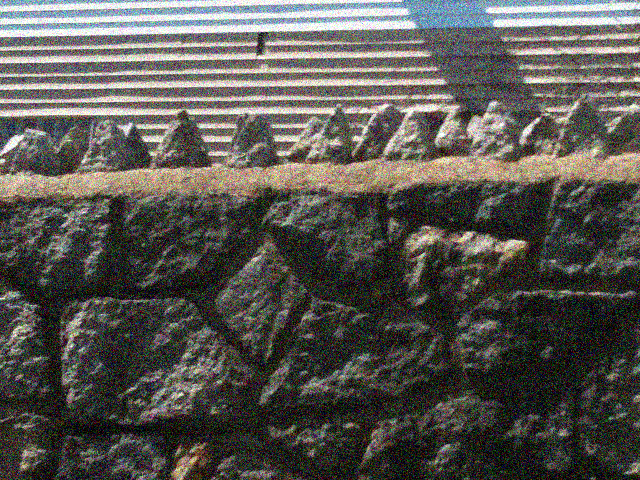
\includegraphics[width=.45\textwidth]{StoneWallNoisy164725L001} \label{StoneWallNoisy164725L001}}
\subfigure{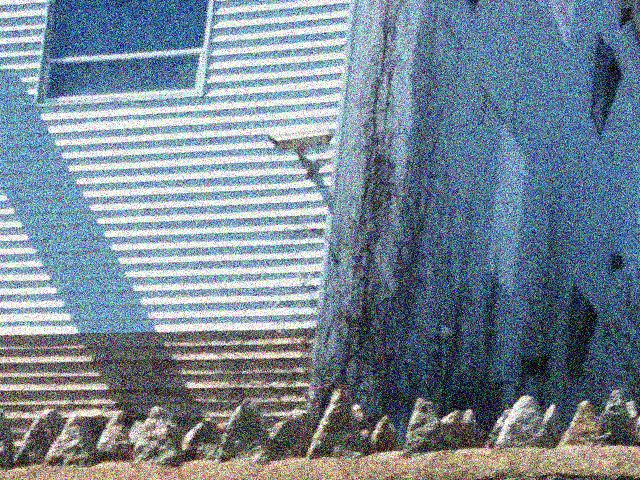
\includegraphics[width=.45\textwidth]{StoneWallNoisy164725R001} \label{StoneWallNoisy164725R001}}
\caption{Stone Wall Views with Average SNR of 16.473 dB (a) Left View, (b) Right View}
\label{StoneWallNoisyImages}
\end{figure}

\begin{figure}
\centering
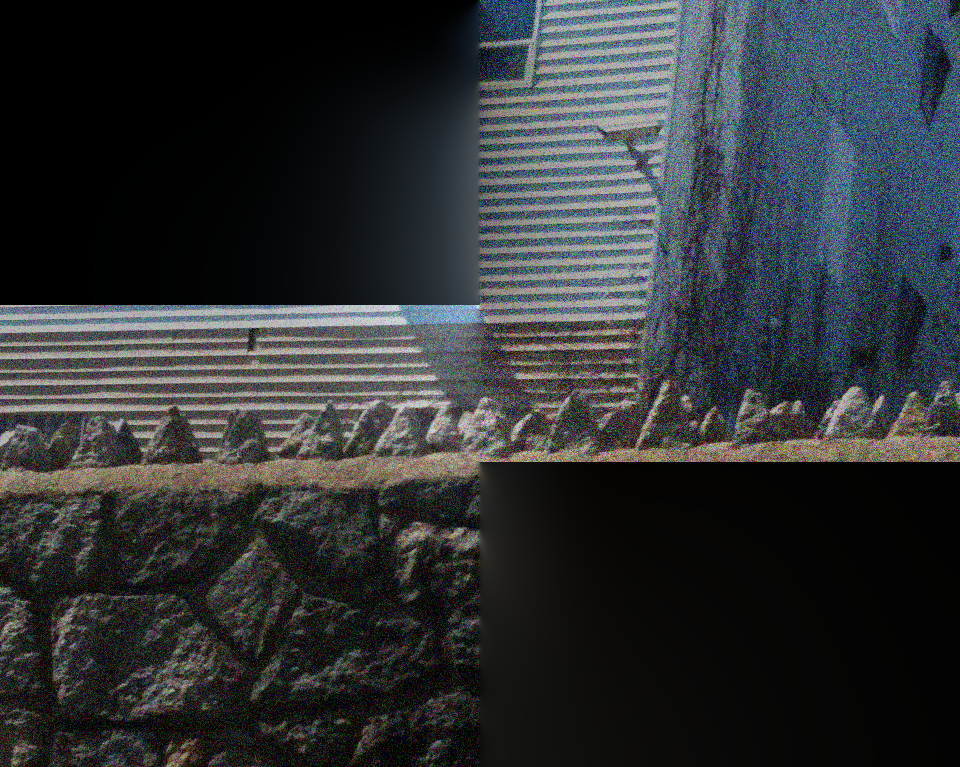
\includegraphics[width=1\textwidth]{StoneWallNoisy164725SP001001}
\caption{Stone Wall Noisy Views Blended (Average SNR: 16.473 dB)}
\label{StoneWallNoisyStitched}
\end{figure}

% STONEWALL SMALL OVERLAP
\begin{figure}
\centering
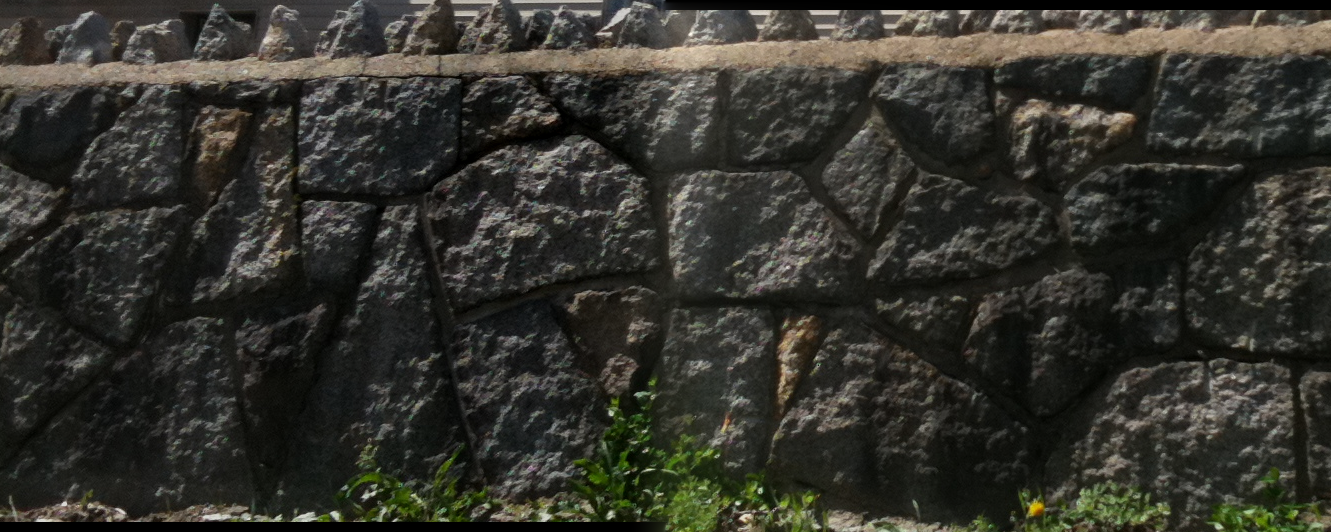
\includegraphics[width=.8\textwidth]{StoneWallSP002002}
\caption{Stone Wall Views Blended with 1\% Overlap}
\label{StoneWallSmall}
\end{figure}

%%%%%%%%%%%%%%%%%%%%%%%%%%%%%%%%%%%%%%%%%%%%%%%%%%%%%%%%%%%%%%%%%%%%%%%%%%%%%%%
% END OF DOCUMENT
